\documentclass[twocolumn,secnumarabic,amssymb, nobibnotes, aps, prl,
superscriptaddress, nobalancelastpage]{revtex4}
\newcommand{\revtex}{REV\TeX\ }
\newcommand{\classoption}[1]{\texttt{#1}}
\newcommand{\macro}[1]{\texttt{\textbackslash#1}}
\newcommand{\m}[1]{\macro{#1}} \newcommand{\env}[1]{\texttt{#1}}
\setlength{\textheight}{9.5in} \usepackage{graphicx}
\setlength{\belowcaptionskip}{6pt}
\usepackage{amsmath} \usepackage{braket} \usepackage{epsfig}
\usepackage{upgreek}
\usepackage{textcomp}
\usepackage[free-standing-units]{siunitx}

\newcolumntype{N}{>{\centering\arraybackslash}m{1.3in}}
\newcolumntype{M}{>{\centering\arraybackslash}m{1.0in}}
\newcolumntype{G}{>{\centering\arraybackslash}m{0.5in}}
\newcolumntype{R}{>{\raggedleft\arraybackslash}m{0.4in}}

\newcommand{\tot}{\ensuremath{\sigma_{tot}}}
\newcommand{\totRD}{\ensuremath{\sigma_{A,A'}}(E)}
\newcommand{\react}{\ensuremath{\sigma_{react}}}
\newcommand{\elast}{\ensuremath{\sigma_{el}}}

\newcommand{\oSix}{\ensuremath{^{16}}O}
\newcommand{\oSeven}{\ensuremath{^{17}}O}
\newcommand{\oEight}{\ensuremath{^{18}}O}
\newcommand{\oSixEight}{\ensuremath{^{16,18}}O}

\newcommand{\neEight}{\ensuremath{^{18}}N\lowercase{e}}

\newcommand{\caForty}{\ensuremath{^{40}}C\lowercase{a}}
\newcommand{\caEight}{\ensuremath{^{48}}C\lowercase{a}}
\newcommand{\caAughtEight}{\ensuremath{^{40,48}}C\lowercase{a}}

\newcommand{\niSix}{\ensuremath{^{56}}N\lowercase{i}}
\newcommand{\niEight}{\ensuremath{^{58}}N\lowercase{i}}
\newcommand{\niSixty}{\ensuremath{^{60}}N\lowercase{i}}
\newcommand{\niOne}{\ensuremath{^{61}}N\lowercase{i}}
\newcommand{\niTwo}{\ensuremath{^{62}}N\lowercase{i}}
\newcommand{\niFour}{\ensuremath{^{64}}N\lowercase{i}}
\newcommand{\niEightFour}{\ensuremath{^{58,64}}N\lowercase{i}}
\newcommand{\niNat}{\ensuremath{^{\text{nat}}}N\lowercase{i}}

\newcommand{\rhThree}{\ensuremath{^{103}}R\lowercase{h}}

\newcommand{\snTwelve}{\ensuremath{^{112}}S\lowercase{n}}
\newcommand{\snFourteen}{\ensuremath{^{114}}S\lowercase{n}}
\newcommand{\snFifteen}{\ensuremath{^{115}}S\lowercase{n}}
\newcommand{\snSixteen}{\ensuremath{^{116}}S\lowercase{n}}
\newcommand{\snSeventeen}{\ensuremath{^{117}}S\lowercase{n}}
\newcommand{\snEighteen}{\ensuremath{^{118}}S\lowercase{n}}
\newcommand{\snNineteen}{\ensuremath{^{119}}S\lowercase{n}}
\newcommand{\snTwenty}{\ensuremath{^{120}}S\lowercase{n}}
\newcommand{\snTwo}{\ensuremath{^{122}}S\lowercase{n}}
\newcommand{\snFour}{\ensuremath{^{124}}S\lowercase{n}}
\newcommand{\snTwelveFour}{\ensuremath{^{112,124}}S\lowercase{n}}
\newcommand{\snNat}{\ensuremath{^{\text{\lowercase{nat}}}}S\lowercase{n}}
\newcommand{\snTwelveNatFour}{\ensuremath{^{112,\text{nat},124}}S\lowercase{n}}

\newcommand{\pbEight}{\ensuremath{^{208}}P\lowercase{b}}
\newcommand{\pbNat}{\ensuremath{^{\text{\lowercase{nat}}}}P\lowercase{b}}

% shell labels
\newcommand{\sOne}{s\ensuremath{_{\frac{1}{2}}}}
\newcommand{\pThree}{p\ensuremath{_{\frac{3}{2}}}}
\newcommand{\pOne}{p\ensuremath{_{\frac{1}{2}}}}
\newcommand{\dFive}{d\ensuremath{_{\frac{5}{2}}}}
\newcommand{\dThree}{d\ensuremath{_{\frac{3}{2}}}}
\newcommand{\fSeven}{f\ensuremath{_{\frac{7}{2}}}}
\newcommand{\fFive}{f\ensuremath{_{\frac{5}{2}}}}
\newcommand{\gNine}{g\ensuremath{_{\frac{9}{2}}}}
\newcommand{\gSeven}{g\ensuremath{_{\frac{7}{2}}}}
\newcommand{\hEleven}{h\ensuremath{_{\frac{11}{2}}}}

\newcommand{\tZero}{T\ensuremath{_{0}}}

\begin{document}

\begin{abstract}
    The neutron total cross sections \tot\ of $^{16,18}$O,
    $^{58,nat,64}$Ni, $^{103}$Rh, and $^{112,nat,124}$Sn have been measured at the Los Alamos
    Neutron Science Center (LANSCE) at intermediate energies (3 $\leq E_{n}
    \leq$ 450 MeV) by
    leveraging waveform digitizer technology. The results are in good agreement
    with previous measurements that used analog techniques,
    excepting small deviations at high energies. These data
    continue the campaign of
    \tot\ measurements we initiated with the case study of $^{40,48}$Ca in 2009.
    The \tot\ relative differences between isotopes are presented,
    revealing additional information about
    the isovector components needed for an accurate optical model (OM)
    description away from stability. Digitizer-enabled \tot-measurement
    techniques are discussed and a Dispersive Optical Model (DOM)
    analysis using these data to extract neutron skins and spectroscopic factors
    is presented.
\end{abstract}

\title{Isotopically-Resolved Neutron Total Cross Sections At
Intermediate Energies}

\author{C.~D.~Pruitt}  \email[Corresponding author:]{cdpruitt@wustl.edu}
\author{R.~J.~Charity}
\author{D. E.~M.~Hoff}  
\author{L.~G.~Sobotka}
\author{K.~W.~Brown} \altaffiliation{Present Address: \textit{National
        Superconducting Cyclotron Laboratory, Departments of Physics and
Astronomy, Michigan State University, East Lansing, MI 48824, USA}}
\author{J.~M.~Elson}
\affiliation{Department of Chemistry, Washington University, St. Louis, MO 63130}

\author{H. Y. Lee}
\author{M. Devlin}
\author{N. Fotiadis}
\author{S. Mosby}
\affiliation{Los Alamos National Lab, Los Alamos, NM 87545, USA}
\maketitle

\section{Supplemental Materials}

\begin{figure}
    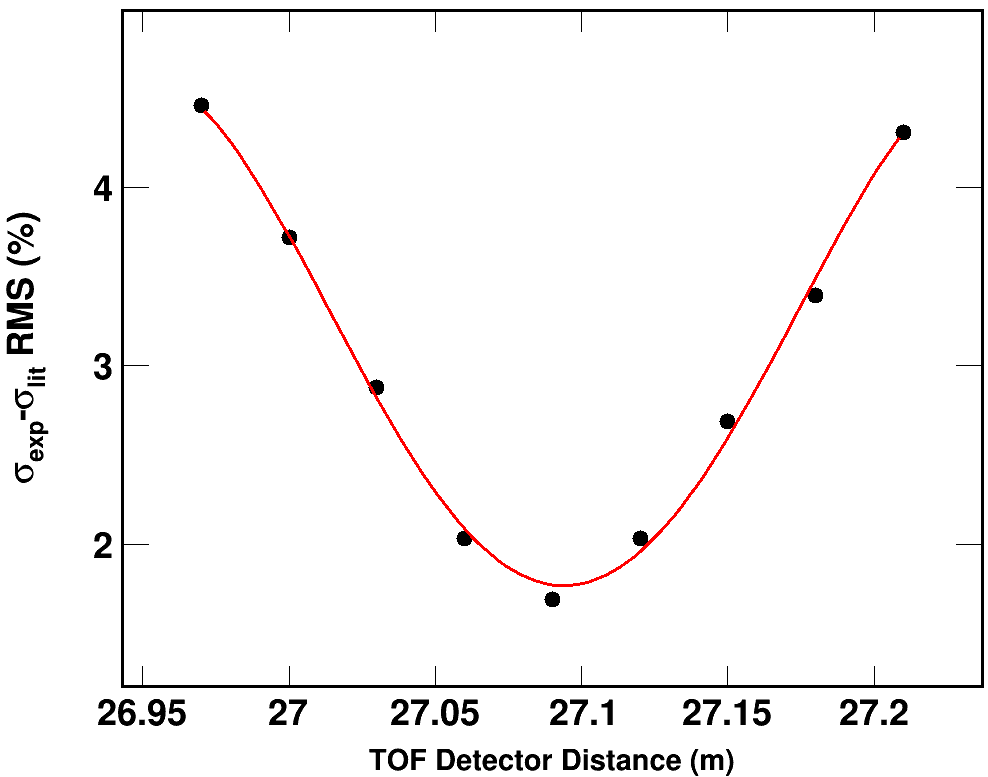
\includegraphics[width=0.5\textwidth]{figures/DistanceStudyNi.png}
    \caption{(Color online) Results of a study to determine the distance between
    the neutron source and the TOF detector for the Ni/Rh running configuration
are shown. First, a plausible range of flight path distances (26.97-27.21 m) was
selected based on rough estimation during the experiment. Using each
distance in this range, the \tot\ for natural carbon was calculated in the
resonance region (3-15 MeV). The RMS difference between the cross section
generated using that distance and literature data from Abfalterer
\cite{Abfalterer2000, Abfalterer2001} was calculated (shown as black points in
the figure). A quartic fit to these RMS data is shown (solid line). By minimizing the
RMS difference, the flight path distance was determined as 2709$\pm$1 cm for the
Ni/Rh run configuration and 2554$\pm$1 cm for the Sn/O run configuration.}
    \label{DistanceStudy}
\end{figure}

\begin{figure}
    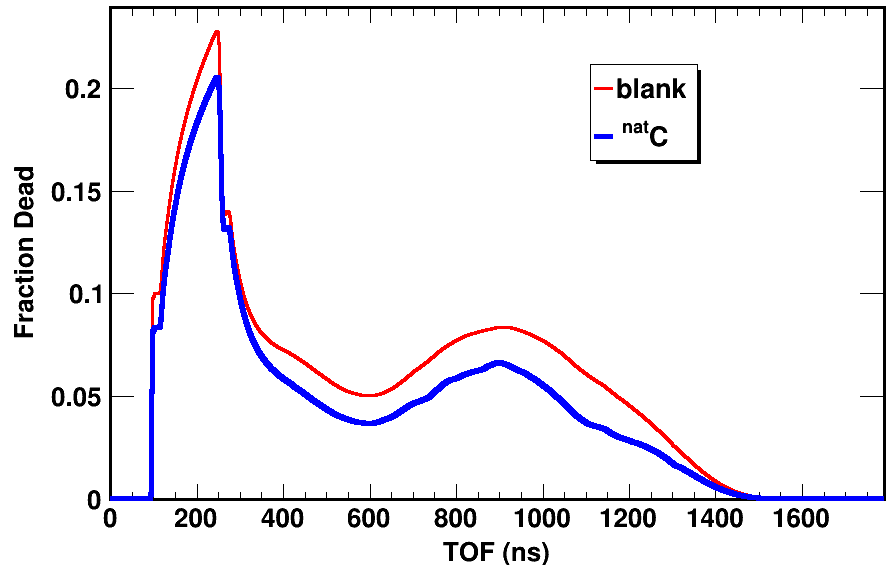
\includegraphics[width=0.5\textwidth]{figures/exampleDeadtimeSpectrum.png}
    \caption{(Color online) Using TOF data from a typical run, the probability that a given 
        TOF bin is ``dead" is shown for the blank sample (dashed line) and the $^{\text{nat}}$C   
        sample (solid line). The sharp rise at 90 ns is the response to the
        $\gamma$-ray flash, the gradual increase from 90-245 ns is the response to
        the arrival of high-energy neutrons, and the sharp fall at 245 ns
        is the elapse of the $\gamma$-ray ``shadow". Only high-energy neutrons
        have a probability-dead exceeding 10\%.
    }
    \label{ExampleDeadtimeSpectrum}
\end{figure}

\begin{figure}
    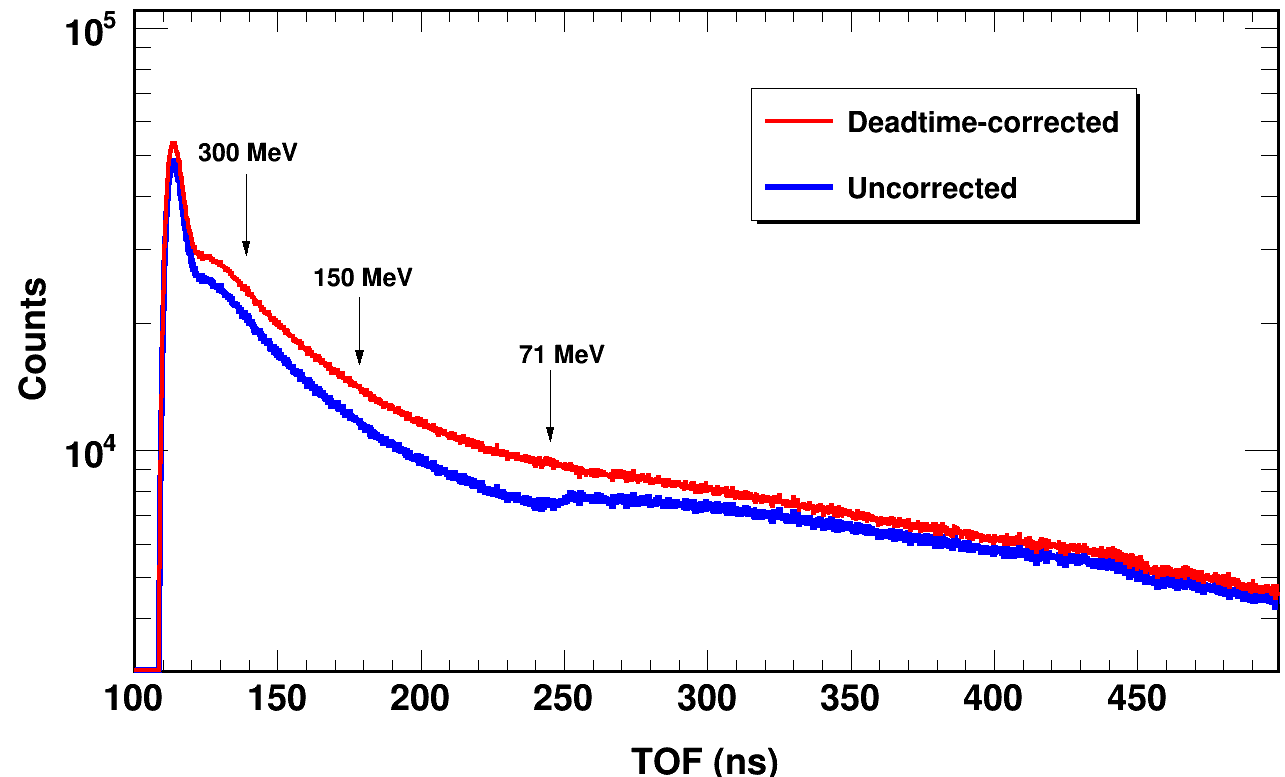
\includegraphics[width=0.5\textwidth]{figures/CorrectionEffectOnTOF.png}
    \caption{(Color online) A typical TOF spectrum from the Ni/Rh
        run configuration is shown, before (in blue) and after (in red) analytic
        deadtime correction. Relevant neutron energies are indicated above the spectra.
        For this digitizer configuration, the mean deadtime was 155 ns (see Fig.
        \ref{TimeDifferenceBetweenEvents} for details on mean deadtime determination).
        Note that at 245 ns, there is an
        obvious defect in the uncorrected spectrum is repaired in the corrected
        spectrum. The defect
        corresponds to the elapse of the 155-ns-long deadtime ``shadow" from the $\gamma$-ray
        flash, which arrived at 90 ns (not shown).
    }
    \label{CorrectionEffectOnTOF}
\end{figure}

\begin{figure}
    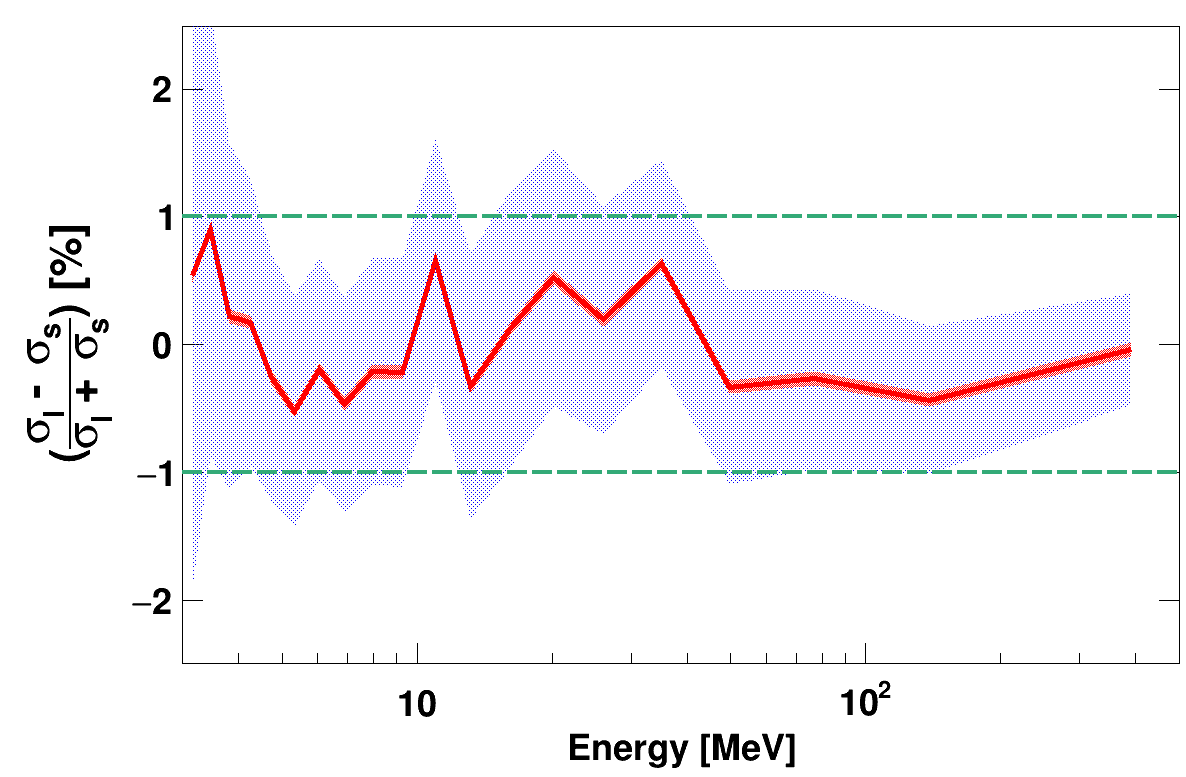
\includegraphics[width=0.5\textwidth]{figures/relativeDiff_longCarbonShortCarbon.png}
    \caption{(Color online) Relative difference of cross sections (red line) of
        our two lengths of $^{\text{nat}}$C, (27.3 mm and 13.7 mm), shown from 3-400
        MeV. Total error
        (including statistical and systematic) is indicated by the blue
        dotted region. Systematic error only (due to uncertainty in the areal
        density) is shown by the red hatched region (very small and immediately adjacent to 
        the red line). Clearly, statistical error dominates for this relative
        difference.
        Despite the low statistics of this diagnostic run (only 1.5 hours
        beam-on-target for each sample), the high efficiency of the
        digitizer-enabled approach means that the relative difference can be resolved to 
        $\pm$1\% for most of the energy range.
    }
    \label{CarbonBenchmarking}
\end{figure}

\begin{figure}
    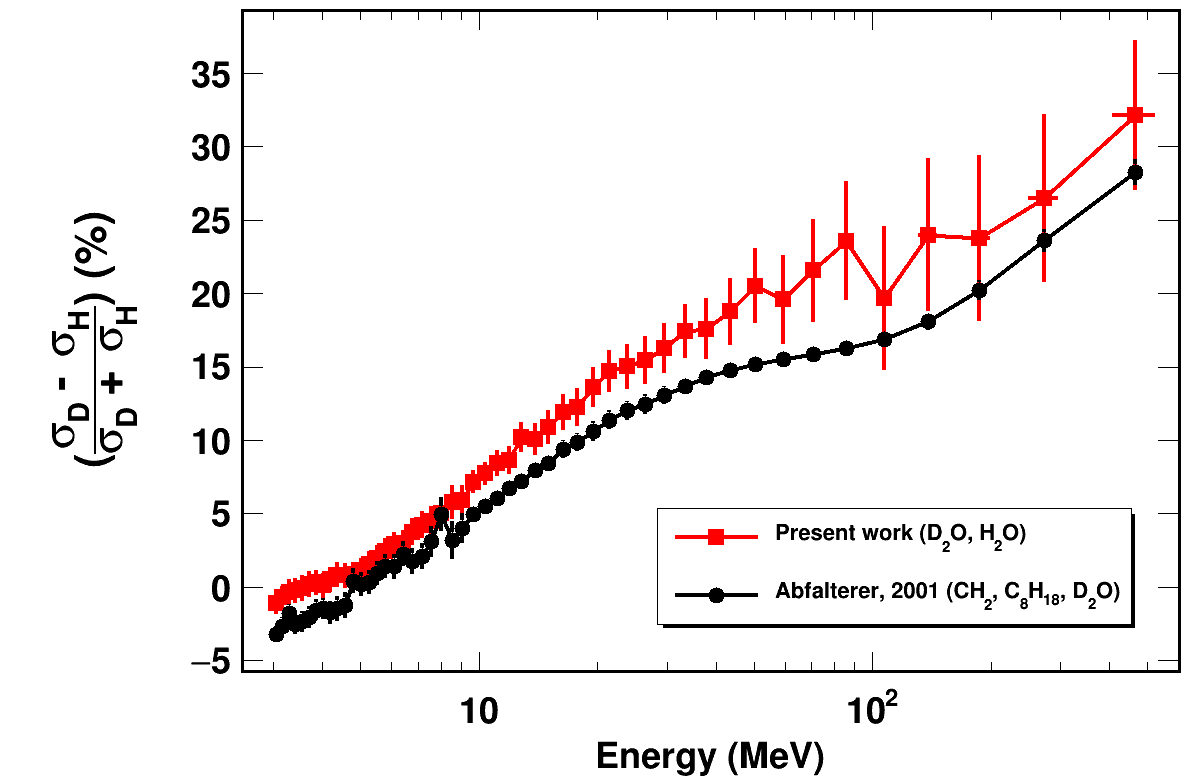
\includegraphics[width=0.5\textwidth]{figures/relativeDiff_DtoH.png}
    \caption{(Color online) Relative difference of cross sections of
        deuterium to hydrogen, as calculated by subtraction of our O \tot\ from
        D$_{2}$O and H$_{2}$O. Our results are shown in red. For comparison, the D/
        H relative difference measurement of
        Abfalterer et al. \cite{Abfalterer1998}, which used hydrocarbon and
    D$_{2}$O samples, is shown in black. The systematic 2-3\% difference between
the two data sets is comparable to the 2\% systematic difference between our
\oSix\ absolute neutron \tot\ results and those of \cite{Abfalterer2001}.
}
    \label{DtoH}
\end{figure}

\end{document}
